\section{Generics}
Generics können in Klassen, Structs und Delegates verwendet werden. Generics sind für Value Types schneller, bei Reference Type jedoch nicht (Verglichen mit object). Die hat den Grund, dass kein Boxing und Unboxing verwendet wird. Vorteile: Hohe Wiederverwendbarkeit, Typensicherheit, Performance. Hauptanwendungsfall sind die Collections.

\subsection{Type Constraints}
Mit dem Keyword where kann eine Regel definiert werden, die der dynamische Typ erfüllen muss.
\begin{figure}[h!]
	\centering
  	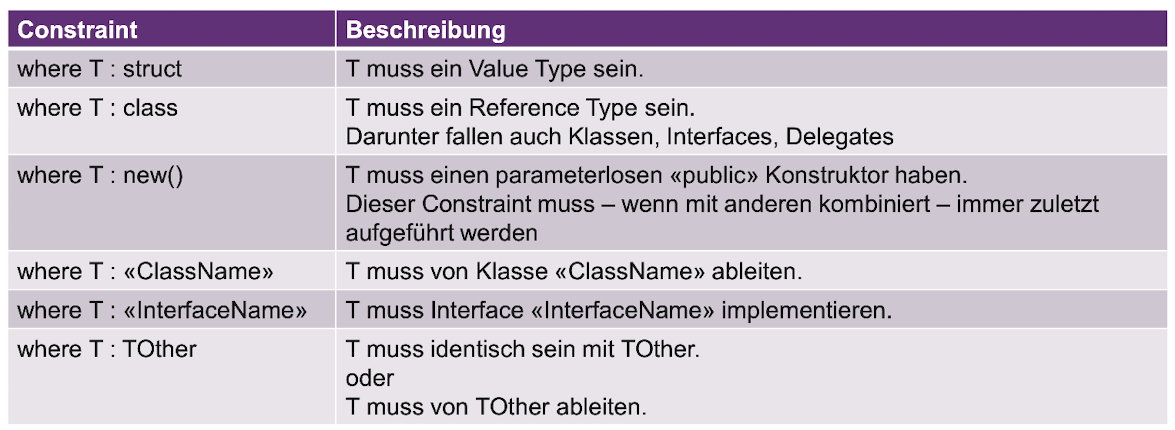
\includegraphics[width=0.75\textwidth]{typeconstraints}
    \caption{Type Constraints}
\end{figure}

\subsection{Vererbung}
 Generische Klassen können von anderen generischen Klassen erben. 
 
 \subsection{Nullable Types}
 \begin{itemize}
  \itemsep -0.5em 
  \item Der "?" Operator erlaubt es NULL werte einem Wertetype zuzuweisen. Der Typ ist dann $Nullable<T>$
  \item Arithemtische Ausdrücke mit Null sind immer false, ausser "null == null"
  \item Der "??" Operator erlaubt es einen Default Wert anzugeben, falls die Variable leer ist.
\end{itemize}
